\cmark\ An atomic hydrogen beam was formed by photodissociating H$_2$S.


\vspace{-8mm}

\begin{figure}[h]
    \centering
    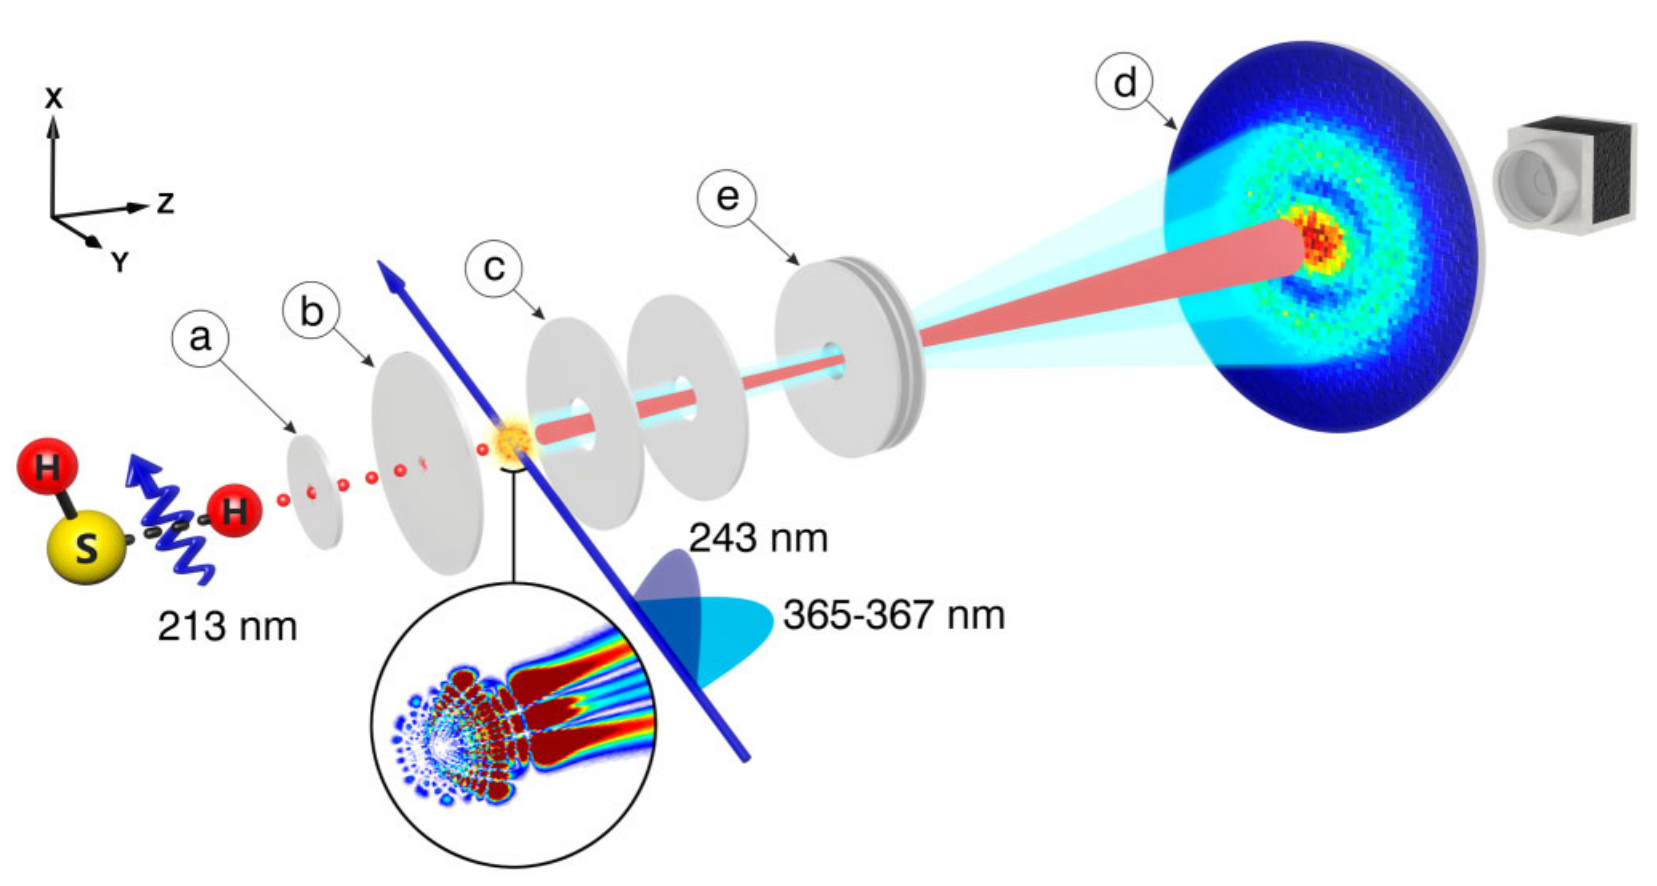
\includegraphics[width=0.75\textwidth]{figures/2.png}
    %\caption{}
    %\label{fig:}
\end{figure}

\vspace{-4mm}

\cmark\ The ground state hydrogen atoms were ionized into a highly excited Rydberg state.
% в котором орбиталь обычно далеко от центрального ядра

\cmark\ By applying a voltage difference across the repeller (b) and extractor (c) electrodes, the
photoelectrons were accelerated towards a two-dimensional detector (d).

